\section{Feasibility of Routing Around Nation-States}
\label{avoid_results}

We now explore the extent to which overlay networks can improve path diversity and help clients 
route around specific countries.  In this section, we develop an avoidance metric and algorithm, and
evaluate the effectiveness of overlay nodes to avoid specific countries.

\subsection{Measurement Approach}
\label{avoid_pipelines}

An overlay network of relay nodes can
help clients route around countries or access content 
that is hosted in a different country; this section performs measurements to evaluate
the feasibility of such an approach. Figure~\ref{fig:avoidance_relays}
shows the steps in our measurement experiment.
After selecting potential relay nodes, we perform traceroute measurements from
the country of origin to each relay (1',2'), and from each relay to the set of top 100 domains
in the original country (1,2,3). We
then analyze these traceroutes using the approach shown in Figure~\ref{fig:analysis_pipeline}
to determine the resulting country-level paths. 

\begin{figure}[t]
\centering
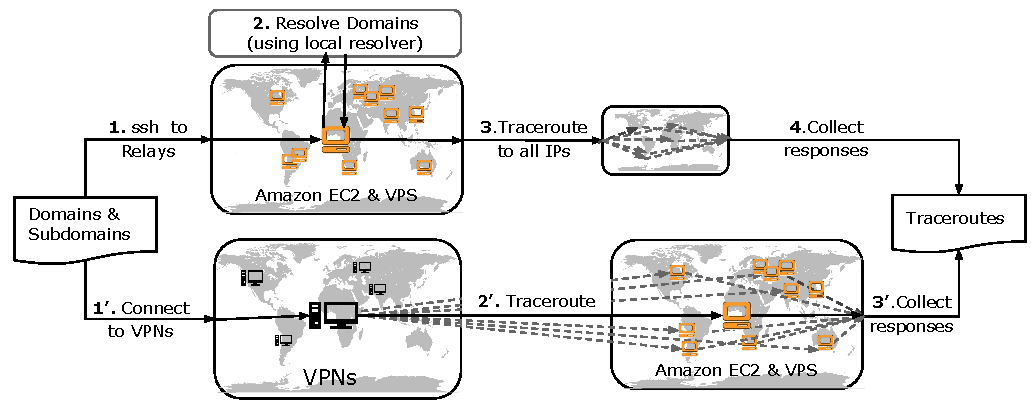
\includegraphics[width=.5\textwidth]{Country-Avoidance-Relays}
\caption{Measurement approach for country avoidance with overlay network relays.}
\label{fig:avoidance_relays}
\end{figure}

We use eight EC2 instances, one in each region
(United States, Ireland, Germany, Singapore, South Korea, Japan, Australia,
Brazil), as well as four Virtual Private Server (VPS) machines (France,
Spain, Brazil, Singapore), which are virtual machines.
% that are functionally equivalent to dedicated physical servers.  
Combining these two sets of machines allows us to evaluate country avoidance with a diverse set of relays. 

\subsection{Avoidability Metrics}
\label{metrics}

We introduce a new metric, avoidability, to measure how often a client in
one country can avoid another specific country.
Using the proposed metric
and algorithm, we can compare how well the different methods achieve
country avoidance for any (X, Y) pair.

{\bf Avoidability metric.}  We introduce an avoidability metric to
quantify how often
traffic can avoid Country Y when it originates in Country X.
Avoidability reflects the fraction of paths that originate in Country
X and do not transit Country Y.  We calculate this value by dividing the
number of paths from Country X to domains that do not traverse Country Y
by the total number of paths from Country X. The resulting value is
in the range [0,1], where 0 means the country is unavoidable for all of
the domains in our study, and 1 means the client can avoid Country Y for
all domains in our study.  For example, there are three paths
originating in Brazil: (1)~$BR \rightarrow US$, (2)~$BR \rightarrow CO
\rightarrow None$, (3)~$BR \rightarrow *** \rightarrow BR$.  After
processing the paths as described in Section~\ref{c_map}, the resulting
paths are: (1)~$BR \rightarrow US$, (2)~$BR \rightarrow CO$, (3)~$BR
\rightarrow BR$.  The avoidance value for avoiding the United States
would be 2/3 because two out of the three paths do not traverse the
United States.  This metric represents a lower bound,
because it is possible that the third path timed out ($***$) because it
traversed the United States, which would make the third path: $BR
\rightarrow US \rightarrow BR$, and would cause the avoidance metric to
drop to 1/3.

{\bf Avoidability algorithm with relays.}  Measuring the avoidability of Country Y
from a client in Country X using relays entails two components: (1)~Is Country Y
on the path from the client in Country X to the relay?  (2)~Is Country Y on
the path from the relay to the domain?  For every domain, our algorithm checks
if there exists at least one path from the client in Country X through any
relay and on to the domain, and does not transit Country Y.   The algorithm
 produces a value in the range [0,1] that can be
compared to the output of the avoidability metric.

{\bf Upper bound on avoidability.}  Although the avoidability metric
provides a way to quantify how avoidable Country Y is for a client in Country
X, some domains may be hosted only in Country Y, so the avoidance value  would
never reach 1.0.  For this reason, we measured the {\em upper bound} on
avoidance for a given pair of (Country X, Country Y) that represents the best
case value for avoidance.  This algorithm analyzes the destinations of all
domains from all relays and if there exists at least one destination for a
domain that is not in Country Y, then this increases the upper bound value. An
upper bound of 1.0 means that every domain that we measured is hosted (or has
a replica) outside of Country Y.  This value puts the avoidance values in
perspective for each (Country X, Country Y) pair.

\subsection{Results}

We examine the
effectiveness of relays for country avoidance, as well as for keeping local
traffic local.  Table \ref{tab:avoid} shows avoidance values; the top
row shows the countries we studied and the left column shows the country
that the client aims to avoid.
%
Table \ref{tab:avoid} shows two trends: (1)~the ability
for a client to avoid a given Country Y increases with the use of relays; and (2)~certain
countries such as the United States, the United Kingdom, and other countries that
are known to perform interference on traffic are also often the most difficult countries
to avoid.

%\newcolumntype{d}[1]{D{.}{.}{#1}}
\begin{table*}[t]
\tiny
\centering
\resizebox{.95\textwidth}{!}{%
\renewcommand{\arraystretch}{0.75}% Tighter
\begin{tabular}{P{32mm}|d{3.2}d{3.2}|d{3.2}d{3.2}|d{3.2}d{3.2}|d{3.2}d{3.2}|d{3.2}d{3.2}}
\multicolumn{1}{l}{}    & \headrow{No Relay} & \headrow{Relays} & \headrow{No Relay}  & \headrow{Relays} & \headrow{No Relay}  & \headrow{Relays}   & \headrow{No Relay}  & \headrow{Relays}  & \headrow{No Relay} & \headrow{Relays} \\ \toprule
\textit{Country to Avoid}    &\multicolumn{2}{c|}{\textit{Brazil}}   &\multicolumn{2}{c|}{\textit{Netherlands}}   &\multicolumn{2}{c|}{\textit{India}} &\multicolumn{2}{c|}{\textit{Kenya}} &\multicolumn{2}{c}{\textit{United States}}\\ \toprule

Brazil               &0.00     &0.00     &1.00  &1.00   &1.00    &1.00   &1.00  &1.00  &1.00  &1.00  \\ \midrule
Canada               &.98    &1.00     &.99 &1.00   &.98  &.98  &.99  &.99  &.92  &1.00  \\
United States        &\cellcolor[HTML]{F7BE81}.15  &\cellcolor[HTML]{F7BE81}.62     &\cellcolor[HTML]{F7BE81}.41 &\cellcolor[HTML]{F7BE81}.63   &\cellcolor[HTML]{F7BE81}.28  &\cellcolor[HTML]{F7BE81}.65  &\cellcolor[HTML]{F7BE81}.38  &\cellcolor[HTML]{F7BE81}.40  &\cellcolor[HTML]{F7BE81}0.00 &\cellcolor[HTML]{F7BE81}0.00  \\ \midrule
France               &.94  &1.00     &.89 &.99   &.89 &1.00  &.77 &.98  &.89 &.99  \\
Germany              &.99 &1.00     &.95 &.99   &.96  &.99  &.95 &1.00  &.99 &1.00  \\
Great Britain        &.97  &1.00     &.86 &.99   &\cellcolor[HTML]{F7BE81}.79  &\cellcolor[HTML]{F7BE81}1.00  &\cellcolor[HTML]{F7BE81}.50  &\cellcolor[HTML]{F7BE81}.97  &.99 &1.00  \\
Ireland              &.97  &.99     &.89 &.99   &.96 &.99  &.86 &.99  &.99 &.99  \\
Netherlands          &.98  &.99     &0.00 &0.00   &.87  &.99  &\cellcolor[HTML]{F7BE81}.74  &\cellcolor[HTML]{F7BE81}.99  &.97 &.99  \\
Spain                &.82  &1.00     &.99 &.99   &1.00  &1.00  &1.00  &1.00  &1.00 &1.00  \\ \midrule
Kenya                &1.00  &1.00     &1.00 &1.00   &1.00  &1.00  &0.00 &0.00  &1.00 &1.00  \\
Mauritius            &1.00  &1.00     &1.00 &1.00   &1.00  &1.00  &\cellcolor[HTML]{F7BE81}.67 &\cellcolor[HTML]{F7BE81}.99  &1.00 &1.00  \\
South Africa         &1.00  &1.00     &1.00 &1.00   &1.00 &1.00  &\cellcolor[HTML]{F7BE81}.66 &\cellcolor[HTML]{F7BE81}.66  &1.00 &1.00  \\ \midrule
United Arab Emirates &1.00  &1.00     &1.00 &1.00   &1.00 &1.00  &\cellcolor[HTML]{F7BE81}.84 &\cellcolor[HTML]{F7BE81}.99  &1.00 &1.00  \\
India                &1.00  &1.00     &.99 &1.00   &0.00 &0.00  &.94 &1.00  &.99 &1.00  \\
Singapore            &.99  &1.00     &.99 &1.00   &\cellcolor[HTML]{F7BE81}.73  &\cellcolor[HTML]{F7BE81}.94  &.96 &1.00  &.99 &1.00  \\\midrule
\end{tabular}
}
\caption{Avoidance values for using overlay network relays to avoid different countries.  The upper bound on avoidance is 1.0 in most cases, but not all.  It is 
common for some European countries to host a domain, and therefore the upper bound is slightly lower than 1.0.  The upper bound on avoidance of the 
U.S. is significantly lower than for any other country; .886, .790, .844, and .765 are the upper bounds on avoidance 
of the U.S. for paths originating in Brazil, Netherlands, India, and Kenya, respectively.}
\label{tab:avoid}
\end{table*}

\begin{finding}[Relay Effectiveness]
For 84\% of the (Country X, Country Y) pairs shown in Table \ref{tab:avoid} the avoidance with relays reaches the upper bound on avoidance. 
\end{finding}
\noindent
In almost every (Country X, Country Y) pair, where Country X is the
client's country (Brazil, Netherlands, India, Kenya, or the United
States) and Country Y is the country to avoid, the use of an overlay
network makes Country Y more avoidable than the default routes.  The one
exception we encountered is when a client is located in Kenya and wants
to avoid South Africa, where, as mentioned, all paths through our
relays exit Kenya via South Africa.

\begin{finding}[Relays Achieve Upper Bound]
Clients in the U.S. can achieve the upper bound of avoidance for all
countries---relays help clients in
the U.S. avoid all other Country Y unless the domain is hosted in Country~Y.  
\end{finding}
\noindent
Relays are most effective for clients in the United States.  On the other hand,
it is more rare for (Kenya, Country Y) pairs to achieve the upper bound, showing
it is more difficult for Kenyan clients to avoid a given country.  Relays can still
be effective for clients in Kenya: for example, the default routes to the top 100
domains for Kenyans avoid Great Britain 50\% of the time, but with relays this percentage increases to 97\% of the time, and the upper bound is 98\%.
%Figure \ref{fig:ke_avoidance} shows default avoidance, avoidance with relays, and the upper bound for Kenya; it's clear that despite having the worst position for avoidance out of the studied countries, in most cases the avoidance with relays either reaches or because extremely close to the upper bound.  

\begin{finding}[U.S. is Least Avoidable]
The ability for any country to avoid the U.S. is significantly lower than its ability to avoid any other country in all three situations: without relays, with relays, and the upper bound. 
\end{finding}
%Certain surveillance states discussed in Section \ref{surv} are completely unavoidable a small fraction of time from certain client locations.  France is unavoidable for a small percentage of domains for clients located in the Netherlands, Kenya, and the United States.  Similarly, clients in the Netherlands and Kenya cannot avoid Great Britain for a small fraction of domains.  
\noindent
Despite increasing the ability to avoid the U.S., relays are less
effective at avoiding the U.S. compared to all other Country Y.
Clients in India can avoid the U.S. more often than clients in Brazil,
Netherlands, and Kenya, by avoiding the U.S. for 65\% of paths.  Even
using relays, Kenyan clients can only avoid the U.S. 40\% of the time.  The upper bound for avoiding the U.S. is significantly lower in comparison to other countries.  

\begin{finding}[Keeping Local Traffic Local]
Using relays decreased both the number of tromboning paths, and the
number of countries involved in tromboning paths.
\end{finding}
\noindent
Where there were relays located in one of the five
countries that we studied, we evaluated how well the relays kept local
traffic local.  This evaluation was possible for the U.S. and Brazil.
Tromboning Brazilian paths decreased from 13.2\% without relays to
9.7\% with relays; when relays are used, all tromboning paths go only
to the U.S.  With the relays, we see only 1.3\% tromboning paths for a
U.S. client, compared to 11.2\% without relays.  The 1.2\% of
paths that trombones from the U.S. traverse Ireland.
